\subsection{Pure shift elements}
\label{subsec:pureshift__elements}

\begin{figure}[htbp]
    \centering
    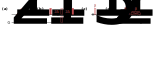
\includegraphics[]{pureshift/elements.png}%
    {\phantomsubcaption\label{fig:pureshift_elements_zs}}%
    {\phantomsubcaption\label{fig:pureshift_elements_bird}}%
    {\phantomsubcaption\label{fig:pureshift_elements_tr}}%
    {\phantomsubcaption\label{fig:pureshift_elements_psyche}}%
    \caption[Pure shift elements]{
        A selection of pure shift elements.
        \textbf{(\subref*{fig:pureshift_elements_zs})} Zangger--Sterk PSE\autocite{Zangger1997JMR}, involving the combination of a selective \ang{180} refocusing pulse and a weak gradient.
        \textbf{(\subref*{fig:pureshift_elements_bird})} BIRD PSE\autocite{Garbow1982CPL,Aguilar2011ACIE}; the delay $\Delta$ is set to $1/(4 \cdot \oneJ{CH})$.
        \textbf{(\subref*{fig:pureshift_elements_tr})} Time-reversal PSE\autocite{Sorensen1985JACS}, simply consisting of a hard pulse with variable flip angle $\beta$. Multiple spectra with different values of $\beta$ must be co-added to suppress artefacts (though this suppression is not perfect, as discussed in the text).
        \textbf{(\subref*{fig:pureshift_elements_psyche})} PSYCHE PSE\autocite{Foroozandeh2014ACIE}, consisting of two saltire pulses\autocite{Foroozandeh2018CEJ,Foroozandeh2020JMR} with flip angle $\beta$, and a weak gradient.
    }
    \label{fig:pureshift_elements}
\end{figure}


\subsubsection{Zangger--Sterk}

We are finally now in a position to study individual PSEs and their mechanisms of action.
We begin with the Zangger--Sterk (ZS, or `slice-selective') PSE\autocite{Zangger1997JMR}, in which a selective refocusing pulse and a weak gradient are simultaneously applied (\cref{fig:pureshift_elements_zs}).
In practice, an rSNOB pulse\autocite{Kupce1995JMRSB} is often used as the refocusing pulse.
The effect of the gradient is to make each spin in the sample have a spatially dependent offset; therefore, in each \textit{slice} (or cross-section) of the sample, a different spin will fall within the specific bandwidth of the refocusing pulse.
This spin is refocused by the PSE and therefore becomes the active spin \textit{within that specific slice}; the bracketing pair of CTP gradients serve to destroy coherences on all the other spins which are not inverted.
Each signal of the pure shift spectrum therefore derives from a specific slice of the sample; during direct detection, all slices simultaneously contribute to the signal, thus yielding a broadband pure shift spectrum.

The sensitivity of the ZS method tends to be low (the factor $c$ tends to be on the order of $0.01$ to $0.05$), as each signal only comes from a narrow section of the sample.
Nevertheless, it still finds wide usage in pure shift applications nowadays, especially because it is compatible with the real-time acquisition mode\autocite{Meyer2013ACIE}: as long as the pulse and the weak gradient are the same each time, then the same active spins will always be chosen in the same slice (as long as diffusion effects are ignored).
The PSE can also be customised through the bandwidth of the refocusing pulse: decreasing this improves the spatial differentiation between spins which have similar intrinsic offsets, yielding better decoupling quality, albeit at the cost of sensitivity.
The ZS element can be easily---and has been---adapted for use in many experiments, including (but not limited to) absorption-mode 2DJ spectroscopy\autocite{Pell2007JMR} and selective refocusing (SERF) experiments for the measurement of $\nJ{HH}$\autocite{Giraud2010ACIE,Gubensak2014CC,Mishra2017JMR,Buchberger2018MRC}.


\subsubsection{BIRD}

Next up is the \textit{bilinear rotation decoupling} (BIRD) pulse element (\cref{fig:pureshift_elements_bird}).
BIRD is not spatially selective like the ZS method; instead, it is \textit{isotope-selective} in that it acts as a \angang{180}{y} pulse on \carbon{}--bound protons, and does not affect \carbont{}--bound protons.
Consequently, all \carbon{}--bound protons become the active spins in the context of pure shift NMR.
The first report of the BIRD element\autocite{Garbow1982CPL}, in 1982, was clearly ahead of its time: it reported the use of an interferogram-type approach to obtain 1D pure shift spectra.
However, in the subsequent decades, this seemed to have been forgotten: BIRD found much more use as an isotope-selective rotation element in heteronuclear NMR\autocite{Uhrin1993JMRSA}, until its use as a pure shift element was `rediscovered'\autocite{Sakhaii2009JMR,Aguilar2011ACIE}.

An immediate drawback of BIRD is that it does not decouple geminal (diastereotopic) \ch{CH2} groups, as both protons would be either both active or both passive.
The sensitivity penalty of BIRD is also relatively severe: the factor $c$ derives from the natural abundance of \carbon{}, which is approximately $0.011$.
However, it is also compatible with real-time acquisition\autocite{Lupulescu2012JMR}, and has found particular success as a pure shift element in the $F_2$ dimension of HMQC and HSQC experiments\autocite{Sakhaii2009JMR,Paudel2013ACIE,Reinsperger2014JMR,Kiraly2018MRC,Nolis2019JMR_psHSQC,Singh2020JMR}: in this case, the use of BIRD leads to no loss of sensitivity as only \carbon{}--bound protons are detected in HSQC experiments anyway.%
\footnote{In fact, the sensitivity is increased by the collapse of multiplet structure.}
It should be noted that the BIRD element does not need to be combined with a hard \ang{180} pulse to form a JRE: the inverse effect of only flipping the passive spins can be accomplished by simply changing the phase of both internal \ang{180} pulses to $+y$.
Using the nomenclature of Uhr{\'i}n et al.,\autocite{Uhrin1993JMRSA} the PSE and JRE forms of the BIRD pulse can be labelled as BIRD\textsuperscript{d,X} and BIRD\textsuperscript{r,X} respectively.

\subsubsection{Time-reversal}

The \textit{time-reversal} PSE (\cref{fig:pureshift_elements_tr}) is even simpler: it consists only of one hard pulse with flip angle $\beta$\autocite{Sorensen1985JACS}.
The catch is that the experiment must be repeated with different values of $\beta$, and the results added up with specific weightings.\autocite{Griesinger1986JCP}
This leads to cancellation of \textit{some}, but not all, of the unwanted coherences: for example, on its own, it does not suppress COSY-type coherence transfer such as $I_{1-}I_{2\alpha} \to I_{1\alpha}I_{2+}$.
This proved to be inconsequential in the original application of $F_1$ decoupling in a 2D NOESY\autocite{Sorensen1985JACS}; however, it is not acceptable in a 1D context as it leads to substantial artefacts.
This will be discussed in more detail in \cref{sec:pureshift__timerev}, so a fuller analysis of the time-reversal PSE is deferred until then.


\subsubsection{PSYCHE}

Finally, we come to the PSYCHE method, which is generally considered the current state of the art for pure shift NMR.\autocite{Foroozandeh2014ACIE}
The corresponding PSE (\cref{fig:pureshift_elements_psyche}) consists of two swept-frequency pulses applied during a weak gradient: for example, a pair of chirps with opposite sweep directions can be used.
The signal-to-artefact ratio of PSYCHE can be further improved by using two \textit{saltire pulses}: these are superpositions of chirps which simultaneously sweep in both frequency directions\autocite{Foroozandeh2018CEJ}.
The operation of this PSE is not easy to fully explain\autocite{Foroozandeh2020JMR}. However, we can adopt the (not fully accurate, but still useful) instant-flip approximation\autocite{Zwahlen1997JACS,Kupce2007JMR}---that the swept-frequency pulse acts as an instantaneous \ang{180} rotation on each frequency it passes through.
Using this, the PSYCHE element (or strictly, the PSYCHE JRE, including a hard \ang{180} pulse) may be viewed as a spatially parallelised version of the anti $z$-COSY experiment\autocite{Oschkinat1986JMR,Pell2007MRC}, which we now describe.
